\documentclass[10pt,a4paper]{article}
\usepackage[right=0.5cm, left=0.5cm,top=1cm,bottom=1.5cm]{geometry}
\usepackage{enumitem}
\usepackage{graphicx}
\usepackage{array, tasks}
\usepackage{blindtext}
\usepackage{fontspec}
\usepackage{amsmath,amsfonts,amssymb,mathrsfs,amsthm}
\usepackage{fancyhdr}
\usepackage{xcolor}
\usepackage{booktabs}
\usepackage[font={bf}]{caption}
% \captionsetup[table]{box=colorbox,boxcolor=orange!20}
\usepackage{float}
\usepackage{esvect}
\usepackage{tabularx}
\usepackage{pifont}
\usepackage{colortbl}
 \usepackage{fancybox}
 \mathversion{bold}
 \usepackage{pgfplots}
 % \usepackage[utf8]{inputenc}
\usepackage{tikz}
 \usepackage[tikz]{bclogo}%
 \usepackage{mathpazo}
\usepackage{ulem}
\usepackage{yagusylo}
\usepackage{textcomp}\usepackage{blindtext}
\usepackage{multicol}
\usepackage{varwidth}
\usetikzlibrary{calc,intersections}
\usepackage{pgfplots}
%\usepackage{fourier}
\pgfplotsset{compat=1.11}
\usepackage{tkz-tab}
\usepackage{xcolor}
\usepackage{color}
\usetikzlibrary{calc}
\mathchardef\times="2202
\usepackage[most]{tcolorbox}
\definecolor{lightgray}{gray}{0.9}
\definecolor{ocre}{RGB}{0,244,244} 
\definecolor{head}{RGB}{255,211,204}
\definecolor{browndark}{RGB}{105,79,56}
%\RequirePackage[framemethod=default]{mdframed}
\usepackage{tikz}
\usetikzlibrary{calc,patterns,decorations.pathmorphing,arrows.meta,decorations.markings}
\usetikzlibrary{arrows.meta}
\makeatletter
\tcbuselibrary{skins,breakable,xparse}
\tcbset{%
  save height/.code={%
    \tcbset{breakable}%
    \providecommand{#1}{2cm}%
    \def\tcb@split@start{%
      \tcb@breakat@init%
      \tcb@comp@h@page%
      \def\tcb@ch{%
        \tcbset{height=\tcb@h@page}%
        \tcbdimto#1{#1+\tcb@h@page-\tcb@natheight}%
        \immediate\write\@auxout{\string\gdef\string#1{#1}}%
        \tcb@ch%
      }%
      \tcb@drawcolorbox@standalone%
    }%
  }%
}
\newcommand{\Lim}{\displaystyle\lim}
\makeatother
\newcommand{\oij}{$\left( \text{O};\vv{i},\vv{j} , \vv{k}\right)$}
\colorlet{darkred}{red!30!black}
\newcommand{\red}[1]{\textcolor{darkred}{ #1}}
\newcommand{\rr}{\mathbb{R}}
\renewcommand{\baselinestretch}{1.2}
 \setlength{\arrayrulewidth}{1.25pt}
\usepackage{titlesec}
\usepackage{titletoc}
\usepackage{minitoc}
\usepackage{ulem}
%--------------------------------------------------------------

\usetikzlibrary{decorations.pathmorphing}
\tcbuselibrary{skins}

%%%%%%%%%%%
%-------------------------------------------------------------------------
\tcbset{
        enhanced,
        colback=white,
        boxrule=0.1pt,
        colframe=brown!10,
        fonttitle=\bfseries
       }
\definecolor{problemblue}{RGB}{100,134,158}
\definecolor{idiomsgreen}{RGB}{0,162,0}
\definecolor{exercisebgblue}{RGB}{192,232,252}
\definecolor{darkbrown}{rgb}{0.4, 0.26, 0.13}

\newcommand*{\arraycolor}[1]{\protect\leavevmode\color{#1}}
\newcolumntype{A}{>{\columncolor{blue!50!white}}c}
\newcolumntype{B}{>{\columncolor{LightGoldenrod}}c}
\newcolumntype{C}{>{\columncolor{FireBrick!50}}c}
\newcolumntype{D}{>{\columncolor{Gray!42}}c}

\newcounter{mysection}
\newcounter{mysubsection}
\newcommand{\mysection}[1]{%
    \stepcounter{mysection} % Increment the counter
    \textcolor{red}{\LARGE\themysection. #1 :}
}
\newcommand{\mysubsection}[2]{
    \stepcounter{mysubsection}
    \textcolor{red}{\large \themysection.#1. #2 :}
}
% \textcolor{red}{\LARGE\bfseries 1. Les équation du deuxiéme degrée :}

%------------------------------------------------------
\newtcolorbox[auto counter]{Definition}{enhanced,
before skip=2mm,after skip=2mm,
colback=yellow!20!white,colframe=lime,boxrule=0.2mm,
attach boxed title to top left =
    {xshift=0.6cm,yshift*=1mm-\tcboxedtitleheight},
    varwidth boxed title*=-3cm,
    boxed title style={frame code={
                        \path[fill=lime]
                            ([yshift=-1mm,xshift=-1mm]frame.north west)  
                            arc[start angle=0,end angle=180,radius=1mm]
                            ([yshift=-1mm,xshift=1mm]frame.north east)
                            arc[start angle=180,end angle=0,radius=1mm];
                        \path[left color=lime,right color = lime,
                            middle color = lime]
                            ([xshift=-2mm]frame.north west) -- ([xshift=2mm]frame.north east)
                            [rounded corners=1mm]-- ([xshift=1mm,yshift=-1mm]frame.north east) 
                            -- (frame.south east) -- (frame.south west)
                            -- ([xshift=-1mm,yshift=-1mm]frame.north west)
                            [sharp corners]-- cycle;
                            },interior engine=empty,
                    },
fonttitle=\bfseries\sffamily,
title={Définition ~\thetcbcounter}}
%------------------------------------------------------
\newtcolorbox[auto counter]{Proposition}{enhanced,
before skip=2mm,after skip=2mm,
colback=yellow!20!white,colframe=blue,boxrule=0.2mm,
attach boxed title to top left =
    {xshift=0.6cm,yshift*=1mm-\tcboxedtitleheight},
    varwidth boxed title*=-3cm,
    boxed title style={frame code={
                        \path[fill=blue]
                            ([yshift=-1mm,xshift=-1mm]frame.north west)  
                            arc[start angle=0,end angle=180,radius=1mm]
                            ([yshift=-1mm,xshift=1mm]frame.north east)
                            arc[start angle=180,end angle=0,radius=1mm];
                        \path[left color=blue,right color = blue,
                            middle color = blue]
                            ([xshift=-2mm]frame.north west) -- ([xshift=2mm]frame.north east)
                            [rounded corners=1mm]-- ([xshift=1mm,yshift=-1mm]frame.north east) 
                            -- (frame.south east) -- (frame.south west)
                            -- ([xshift=-1mm,yshift=-1mm]frame.north west)
                            [sharp corners]-- cycle;
                            },interior engine=empty,
                    },
fonttitle=\bfseries\sffamily,
title={Proposition ~\thetcbcounter}}
%------------------------------------------------------
\newtcolorbox[auto counter]{Theoreme}{enhanced,
before skip=2mm,after skip=2mm,
colback=yellow!20!white,colframe=red,boxrule=0.2mm,
attach boxed title to top left =
    {xshift=0.6cm,yshift*=1mm-\tcboxedtitleheight},
    varwidth boxed title*=-3cm,
    boxed title style={frame code={
                        \path[fill=red]
                            ([yshift=-1mm,xshift=-1mm]frame.north west)  
                            arc[start angle=0,end angle=180,radius=1mm]
                            ([yshift=-1mm,xshift=1mm]frame.north east)
                            arc[start angle=180,end angle=0,radius=1mm];
                        \path[left color=red,right color = red,
                            middle color = red]
                            ([xshift=-2mm]frame.north west) -- ([xshift=2mm]frame.north east)
                            [rounded corners=1mm]-- ([xshift=1mm,yshift=-1mm]frame.north east) 
                            -- (frame.south east) -- (frame.south west)
                            -- ([xshift=-1mm,yshift=-1mm]frame.north west)
                            [sharp corners]-- cycle;
                            },interior engine=empty,
                    },
fonttitle=\bfseries\sffamily,
title={Théorème ~\thetcbcounter}}
%------------------------------------------------------
\newtcolorbox[auto counter]{exemple}{
  % breakable,
  enhanced,
  colback=white,
  boxrule=0pt,
  arc=0pt,
  outer arc=0pt,
  title=Exemple ~\thetcbcounter,
  fonttitle=\bfseries\sffamily\large\strut,
  coltitle=problemblue,
  colbacktitle=problemblue,
  title style={
left color=exercisebgblue,
    right color=white,
    middle color=exercisebgblue  
  },
  overlay={
    \draw[line width=1pt,problemblue] (frame.south west) -- (frame.south east);
    \draw[line width=1pt,problemblue] (frame.north west) -- (frame.north east);
    \draw[line width=1pt,problemblue] (frame.south west) -- (frame.north west);
    \draw[line width=1pt,problemblue] (frame.south east) -- (frame.north east);
  }
}
%----------------------------------------------------
\newtcolorbox[auto counter]{Activite}{
  % breakable,
  enhanced,
  colback=white,
  boxrule=0pt,
  arc=0pt,
  outer arc=0pt,
  title=Activité ~\thetcbcounter,
  fonttitle=\bfseries\sffamily\large\strut,
  coltitle=problemblue,
  colbacktitle=problemblue,
  title style={
left color=yellow!50!white,
    right color=white,
    middle color=yellow!20!white  
  },
  overlay={
    \draw[line width=1pt,problemblue] (frame.south west) -- (frame.south east);
    \draw[line width=1pt,problemblue] (frame.north west) -- (frame.north east);
    \draw[line width=1pt,problemblue] (frame.south west) -- (frame.north west);
    \draw[line width=1pt,problemblue] (frame.south east) -- (frame.north east);
  }
}
%----------------------------------------------------
\newtcolorbox[auto counter]{Application}{
  % breakable,
  enhanced,
  colback=white,
  boxrule=0pt,
  arc=0pt,
  outer arc=0pt,
  title=Application ~\thetcbcounter,
  fonttitle=\bfseries\sffamily\large\strut,
  coltitle=problemblue,
  colbacktitle=problemblue,
  title style={
left color=exercisebgblue,
    right color=white,
    middle color=exercisebgblue  
  },
  overlay={
    \draw[line width=1pt,problemblue] (frame.south west) -- (frame.south east);
    \draw[line width=1pt,problemblue] (frame.north west) -- (frame.north east);
    \draw[line width=1pt,problemblue] (frame.south west) -- (frame.north west);
    \draw[line width=1pt,problemblue] (frame.south east) -- (frame.north east);
  }
}
%----------------------------------------------------
\newtcolorbox{mybox}[2]{enhanced,breakable,
    before skip=2mm,after skip=2mm,
    colback=white,colframe=#2!30!blue,boxrule=0.3mm,rightrule=0.3mm,
    attach boxed title to top center={xshift=0cm,yshift*=1mm-\tcboxedtitleheight},
    varwidth boxed title*=-3cm,
    boxed title style={frame code={
    \path[fill=#2!30!black]
    ([yshift=-1mm,xshift=-1mm]frame.north west)
    arc[start angle=0,end angle=180,radius=1mm]
    ([yshift=-1mm,xshift=1mm]frame.north east)
    arc[start angle=180,end angle=0,radius=1mm];
    \path[draw=black,line width=1pt,left color=#2!1!white,right color=#2!1!blue!65,
    middle color=#2!1!green]
    ([xshift=-2mm]frame.north west) -- ([xshift=2mm]frame.north east)
    [rounded corners=1mm]-- ([xshift=1mm,yshift=-1mm]frame.north east)
    -- (frame.south east) -- (frame.south west)
    -- ([xshift=-1mm,yshift=-1mm]frame.north west)
    [sharp corners]-- cycle;
    },interior engine=empty,
    },
title=#1,coltitle=black,fonttitle=\sffamily}
%---------------------------------------------
\newtcolorbox{boxone}{%
    enhanced,
    colback=brown!10,
    boxrule=0pt,
    sharp corners,
    drop lifted shadow,
    frame hidden,
    fontupper=\bfseries,
    notitle,
    overlay={%
        \draw[Circle-Circle, brown!70!black, line width=2pt](frame.north west)--(frame.south west); 
        \draw[Circle-Circle, brown!70!black, line width=2pt](frame.north east)--(frame.south east);}
    }
    
\begin{document}


\begin{tcolorbox}[title=\textcolor{blue}{\shadowbox{ Prof : Othmane Laksoumi}}
\hfill
\textcolor{blue}{\shadowbox{Calcul vectoriel dans le plan}}]

\end{tcolorbox}

\begin{mybox}{Lycée Qualifiant Zitoun}{gray}
    \begin{minipage}{8cm}
    \textcolor{darkbrown}{Année scolaire : } 2024-2025 \\
    \textcolor{darkbrown}{Niveau : } Tronc commun scientifique \\
    \textcolor{darkbrown}{Durée totale : } $5h$
    \end{minipage}
\end{mybox}

\begin{boxone}
{\Large\ding{45}}
\textcolor{red}{\large Contenus du programme :}
\begin{itemize}
    \item Egalité de deux vecteurs; somme de deux vecteurs; relation de Chasles.
    \item  Multiplication d'un vecteur par un nombre réel.
    \item Colinéarité de deux vecteurs, alignement de trois points.
    \item Définition vectorielle du milieu d'un segment.
premiers
\end{itemize}

{\Large\ding{45}}
\textcolor{red}{\large Les capacités attendues :}
\begin{itemize}
    \item Construire un vecteur de la forme $a\overrightarrow{u} + b\overrightarrow{v}$;
    \item Exprimer les notions et les propriétés de la géométrie affine en utilisant l'outil vectoriel et réciprequement;
    \item Résoudre des problèmes géométriques en utilisant l'outil vectoriel.
\end{itemize}

{\Large\ding{45}}
\textcolor{red}{\large Recommandations pédagogiques :} 
  \begin{itemize}
      \item On rappellera les définitions de la somme de deux vecteurs et de la multiplication d'un vecteur par un nombre réel, on introduira ensuite, à travers des activités simples, les propriétés :
      $(a+b)\overrightarrow{u} = a\overrightarrow{u} + b\overrightarrow{u}$ et $a(\overrightarrow{u} + \overrightarrow{v}) = a\overrightarrow{u} + b\overrightarrow{u}$ et $a.(b\overrightarrow{u}) = (ab).\overrightarrow{u}$.
      \item La multiplication d'un vecteur par un nombre réel doit être liée d'une part, au point $M$ de la droite $(AB)$ qui a pour abscisse $x$ dans le répere $(A,B)$ c'est-à-dire $\overrightarrow{AM} = x\overrightarrow{AB}$, et d'autre part à l'interprétation vectorielle de l'alignement de trois points.
  \end{itemize}
\end{boxone}

\newpage

\begin{tabular}{|>{\raggedright\arraybackslash}p{17cm}|>{\centering\arraybackslash}p{0.8cm}|}
\hline
\rowcolor{head}

\centering Contenu du cours &
 Durée \\
\hline

% \vspace{1cm}
% \rotatebox{90}{Phase de lancement}

% \vspace{1cm}

% \rotatebox{90}{construction de connaissances}
 
\vspace{0.1cm}

\mysection{Egalité de deux vecteurs}
\begin{Definition}
    Soient $A,$ $B,$ $C$ et $D$ quatre points du plan $\mathcal{P}$ tels que $A\neq B$ et $C\neq D$.\\
    On dit que les deux vecteurs $\overrightarrow{AB}$ et $\overrightarrow{DC}$ sont \textcolor{red}{égaux} et on écrit $\overrightarrow{AB} = \overrightarrow{CD}$ lorsque ces deux vecteurs ont :
    \begin{itemize}
        \item la même direction, c'est-à-dire $(AB) // (DC)$
        \item le même sens
        \item la même norme, c'est-à-dire $AB=DC$.
    \end{itemize}
\end{Definition}
\begin{exemple}
    \begin{center}        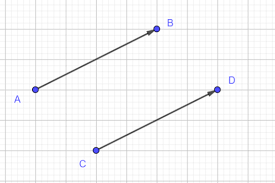
\includegraphics[width=0.5\textwidth]{download.png}
    \end{center}
    On a $\overrightarrow{AB} = \overrightarrow{CD}$ et $\overrightarrow{AB}\neq\overrightarrow{DC}$.
\end{exemple}
\begin{Proposition}
    Soient $A,$ $B,$ $C$ et $D$ quatre points du plan $\mathcal{P}$.\\
    $\overrightarrow{AB} = \overrightarrow{DC}$ si et seulement si $ABCD $ est un parallélogramme.
\end{Proposition}

\begin{exemple}
    Soient $A$, $B$, $C$ et $D$ quatre points tels que : $\overrightarrow{AB}=\overrightarrow{DC}$.\\
    $\overrightarrow{AB}=\overrightarrow{DC}$ signifie que $ABCD$ est un parallélogramme.\\
    Donc $BADC$ et $ADCB$ et $DCBA$ sont des parallélogrammes.\\
    D'où $\overrightarrow{BA} = \overrightarrow{CD}$ et $\overrightarrow{AD} = \overrightarrow{BC}$ et $\overrightarrow{DC} = \overrightarrow{AB}$
\end{exemple}

\begin{Proposition}
    Pour tout vecteur $\overrightarrow{u}$ et tout point $A$ du plan $\mathcal{P}$, il existe un point $B$ tel que : $\overrightarrow{u} = \overrightarrow{AB}$.
\end{Proposition}
\textcolor{red}{Remarque : }\newline
Il existe une infinité de vecteurs égaux à un vecteur donné $\overrightarrow{u}$.\\
\textcolor{red}{Conséquences : }
Quels que soient les points $A$, $M$ et $N$ du plan, on a :
\begin{itemize}
    \item $\overrightarrow{AM} = \overrightarrow{AN}$ signifie que $M=N$.
    \item $\overrightarrow{AM} = -\overrightarrow{MA}$.
    \item $\overrightarrow{AM} = \overrightarrow{0}$ signifie que $M=A$.
    \newline
    Le vecteur $\overrightarrow{0}$ est dit vecteur nul.
\end{itemize}


&\\
\hline

\end{tabular}

\begin{tabular}{|>{\raggedright\arraybackslash}p{17cm}|>{\centering\arraybackslash}p{0.8cm}|}
\hline

\vspace{1mm}
\mysection{Somme de deux vecteurs}
\begin{Definition}
Soient $\overrightarrow{u}$ et $\overrightarrow{v}$ deux vecteurs tels que : $\overrightarrow{u} = \overrightarrow{AB}$ et $\overrightarrow{v} = \overrightarrow{AC}$.\\
La somme des deux vecteurs $\overrightarrow{u}$ et $\overrightarrow{v}$ est le vecteur noté $\overrightarrow{u} + \overrightarrow{v}$ et définie par $\overrightarrow{u} + \overrightarrow{v} = \overrightarrow{AD}$ tel que $ABCD$ est un parallélogramme.\\
\begin{center}
    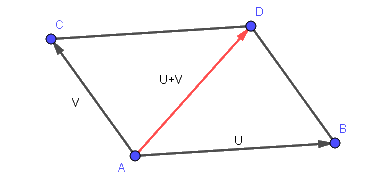
\includegraphics[width=0.5\textwidth]{output-onlinepngtools.png}
\end{center}
\end{Definition}
\begin{Proposition}
\textcolor{red}{Relation de Chasles}\\
Soient $A$, $B$ et $C$ trois points du plan $\mathcal{P}$.
On a $\overrightarrow{AB} + \overrightarrow{BC} = \overrightarrow{AC}$.
\end{Proposition}

\begin{exemple}
    Soient $A$, $B$, $C$, $D$ et $O$ cinq points du plan $\mathcal{P}$.
    \begin{itemize}
        \item Montrons que $\overrightarrow{AC} + \overrightarrow{BD} = \overrightarrow{AD} + \overrightarrow{BC}$.
        \item Montrons que $\overrightarrow{AB} = \overrightarrow{OB} - \overrightarrow{OA}$.
    \end{itemize}
\end{exemple}

\mysection{Multiplication d'un vecteur par un nombre réel}
\begin{Definition}
Soit $\overrightarrow{u}$ un vecteur et $k$ un nombre réel.\\
Le produit du vecteur $\overrightarrow{u}$ par le nombre réel $k$, que l'on note $\overrightarrow{w} = k \overrightarrow{u}$, est défini par :
\begin{itemize}
    \item Si $\overrightarrow{u}$ est un vecteur non nul :
    \begin{itemize}
        \item Si $k = 0$, alors $\overrightarrow{w} = \overrightarrow{0}$ (c'est-à-dire $0.\overrightarrow{u} = \overrightarrow{0}$).
        \item Si $k > 0$, alors $\overrightarrow{w}$ et $\overrightarrow{u}$ ont la même direction, le même sens et $\|\overrightarrow{w}\| = k \|\overrightarrow{u}\|$.
        \item Si $k < 0$, alors $\overrightarrow{w}$ et $\overrightarrow{u}$ ont la même direction, des sens contraires, et $\|\overrightarrow{w}\| = -k\|\overrightarrow{u}\|$.
    \end{itemize}
    \item Si $\overrightarrow{u} = \overrightarrow{0}$, alors $\overrightarrow{w} = \overrightarrow{0}$ (c'est-à-dire $k \overrightarrow{u} = \overrightarrow{0}$).
\end{itemize}
    
\end{Definition}
\begin{exemple}
On considére la figure suivante :
    \begin{center}
        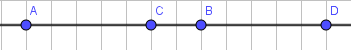
\includegraphics{grille.PNG}
    \end{center}
    \begin{itemize}
        \item Les vecteurs $\overrightarrow{CA}$ et $\overrightarrow{CB}$ ont la même direction, des sens opposés et $CA = 2.5CB$, donc \\$\overrightarrow{CA} = -2.5\overrightarrow{CB}$
        \item  Les vecteurs $\overrightarrow{DA}$ et $\overrightarrow{DB}$ ont la même direction, le même sens et $DA = \displaystyle\frac{12}{5}DB$, donc $\overrightarrow{DA} = \displaystyle\frac{12}{5}\overrightarrow{DB}$.
    \end{itemize}
    
\end{exemple}


&\\
\hline

\end{tabular}

\begin{tabular}{|>{\raggedright\arraybackslash}p{17cm}|>{\centering\arraybackslash}p{0.8cm}|}
\hline

\vspace{1mm}
\begin{Application}
    Soient $A$, $B$, $C$ et $D$ quatre points.\\
    Construire les points $M$, $N$, $P$ définie par :
    \begin{enumerate}
        \item $\overrightarrow{AB} = 2\overrightarrow{AM}$
        \item $\overrightarrow{BC} = -3\overrightarrow{BM}$
        \item $\overrightarrow{CD} = 2.5\overrightarrow{CP}$
    \end{enumerate}
\end{Application}

\begin{Activite}
On considère un vecteur non nul $\overrightarrow{u}$ et on pose $\|\overrightarrow{u}\| = k$.

Soient $a$ et $b$ deux nombres réels tels que $a > 0$, $b < 0$ et $a + b < 0$.\\
$A$, $B$ et $C$ sont des points tels que $\overrightarrow{AB} = a \overrightarrow{u}$ et $\overrightarrow{BC} = b \overrightarrow{u}$.
\begin{enumerate}
    \item Calculer la norme $\|\overrightarrow{AC}\|$ en fonction de $a$, $b$ et $k$.
    \item Montrer que : $(a + b)\overrightarrow{u} = a\overrightarrow{u} + b\overrightarrow{u}$.
\end{enumerate}
\end{Activite}

\begin{Proposition}
    Quels que soient les vecteurs $\overrightarrow{u}$ et $\overrightarrow{v}$ et les réels $a,\ b$ et $k$, on a : 
    \begin{itemize}
        \item $a(\overrightarrow{u} + \overrightarrow{v}) = a\overrightarrow{u} + a\overrightarrow{v}$
        \item $(a+b)\overrightarrow{u} = a\overrightarrow{u} + b\overrightarrow{u}$
        \item $a(b\overrightarrow{u}) = (ab)\overrightarrow{u}$
        \item Si $k\overrightarrow{u} = \overrightarrow{0}$, alors $k=0$ ou $\overrightarrow{u} = \overrightarrow{0}$.
    \end{itemize}
\end{Proposition}

\begin{exemple}
 $\begin{array}{ccc}
        \overrightarrow{V_1} & = & 4(\overrightarrow{u} + \overrightarrow{v}) - 2\overrightarrow{u} \\
         & = & 4\overrightarrow{u} + 4\overrightarrow{v} - 2\overrightarrow{u} \\
         & = & 4\overrightarrow{u} - 2\overrightarrow{u} + 4\overrightarrow{v} \\
         & = & 2\overrightarrow{u} + 4\overrightarrow{v}  \\
         & = & 2(\overrightarrow{u} + 2\overrightarrow{v}) 
         
    \end{array}$
\end{exemple}

\begin{Application}
    Simplifier l'écriture des vecteurs suivants :
    \begin{enumerate}
        \item $\vec{V_1} = 2(\vec{u} + \vec{v}) - 2(\vec{u} - \vec{v})$
        \item $\vec{V_2} = \vec{u} + 2(\vec{u} - \vec{v}) - 3(\vec{u} - \vec{v})$
        \item $\vec{V_3} = 3(\vec{u} - 2\vec{v}) + 5(\vec{v} - \vec{u})$
        \item $\vec{V_4} = \displaystyle\frac{1}{2}(4\vec{u} + 5\vec{v}) - 3\left(\displaystyle\frac{1}{3}\vec{u} + \displaystyle\frac{1}{2}\vec{v}\right)$
    \end{enumerate}
\end{Application}
\mysection{Colinéarité de deux vecteurs :}
\begin{Definition}
    On dit que deux vecteurs $\overrightarrow{u}$ et $\overrightarrow{v}$ sont \textcolor{red}{colinéaires} s'il existe un nombre réel $k$ tel que $\overrightarrow{u} = k\overrightarrow{v}$ ou $\overrightarrow{v} = k\overrightarrow{u}$.
\end{Definition}



&\\
\hline
\end{tabular}

\begin{tabular}{|>{\raggedright\arraybackslash}p{17cm}|>{\centering\arraybackslash}p{0.8cm}|}
\hline

\vspace{1mm}

\begin{Proposition}
    Soient $A,\ B,\ C$ et $D$ quatre points du plan $\mathcal{P}$.
    \begin{itemize}
        \item Les points $A,\ B$ et $C$ sont alignés si et seleument si $\overrightarrow{AB}$ et $\overrightarrow{AC}$ sont colinéaires.
        \item Les droites $(AB)//(CD)$ sont paralléles si et seulement si $\overrightarrow{AB}$ et $\overrightarrow{CD}$ sont colinéaires.
    \end{itemize}
\end{Proposition}

\begin{exemple}
    \begin{center}
        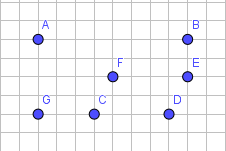
\includegraphics{colineare.PNG}
    \end{center}
    Déterminer tous les vecteurs qui sont colinéaires.
\end{exemple}

\begin{Application}
    Soient $ABCD$ un parallélogramme, $E$ et $F$ les points définis par :
    $$\overrightarrow{CE} = \displaystyle\frac{1}{3}\overrightarrow{CD} \\ \text{ et } \\ \overrightarrow{BF} = \displaystyle\frac{3}{4}\overrightarrow{BE}$$
    \begin{enumerate}
        \item Construire la figure.
        \item Montrer que les points $A,\ C$ et $F$ sont alignés.
    \end{enumerate}
\end{Application}

\mysection{Milieu d'un segment :}
\begin{Proposition}
    Pour qu'un point $I$ soie le milieu du segment $[AB]$, il faut et il suffit que l'une des relations suivantes soit réalisée :
    \begin{enumerate}
        \item $\overrightarrow{AI} = \overrightarrow{IA}$
        \item $\overrightarrow{IA} + \overrightarrow{IB} = \overrightarrow{0}$
        \item $\overrightarrow{AI} = \displaystyle\frac{1}{2}\overrightarrow{AB}$
    \end{enumerate}
\end{Proposition}



&\\
\hline
\end{tabular}

\newpage

\begin{tabular}{|>{\raggedright\arraybackslash}p{17cm}|>{\centering\arraybackslash}p{0.8cm}|}
\hline

\vspace{1mm}
\begin{exemple}
    Soit $ABC$ un triangle.\\
    Construisons les points $E$ et $F$ définis par : 
     $\overrightarrow{BE} = \overrightarrow{BA} + \overrightarrow{BC}$ et $\overrightarrow{AF} = \overrightarrow{AB} + \overrightarrow{AC}$
    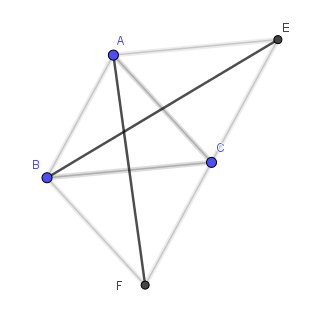
\includegraphics[width=0.3\textwidth]{exemple7.PNG}
    
     Montrons que $C$ est le milieu de $[EF]$.
\end{exemple}




&\\
\hline

\end{tabular}

\end{document}